\section{Question 1 --- Transshipment Network}

\begin{questionbox}
Figure~1 is a transshipment network with four source nodes (1--4), three intermediary nodes
(5--7), and three destination nodes (8--10). The supplies are \(1000\), \(800\), \(1150\), and
\(2050\) units respectively, and the demands are \(1300\), \(2000\), and \(1700\) units respectively.
The unit transportation costs are displayed along each arc in the network.

Based on the transshipment network, complete the following tasks:
\begin{enumerate}
  \item[(a)] Formulate the complete mathematical model for this transshipment network.
  \item[(b)] Construct the standard transportation tableau corresponding to this
        transshipment problem.
  \item[(c)] Use ADBAM to find the initial basic feasible solution.
  \item[(d)] Use the \(uv\) method to find the optimal solution.
\end{enumerate}
\end{questionbox}

\subsection*{Reading the network}
\begin{center}
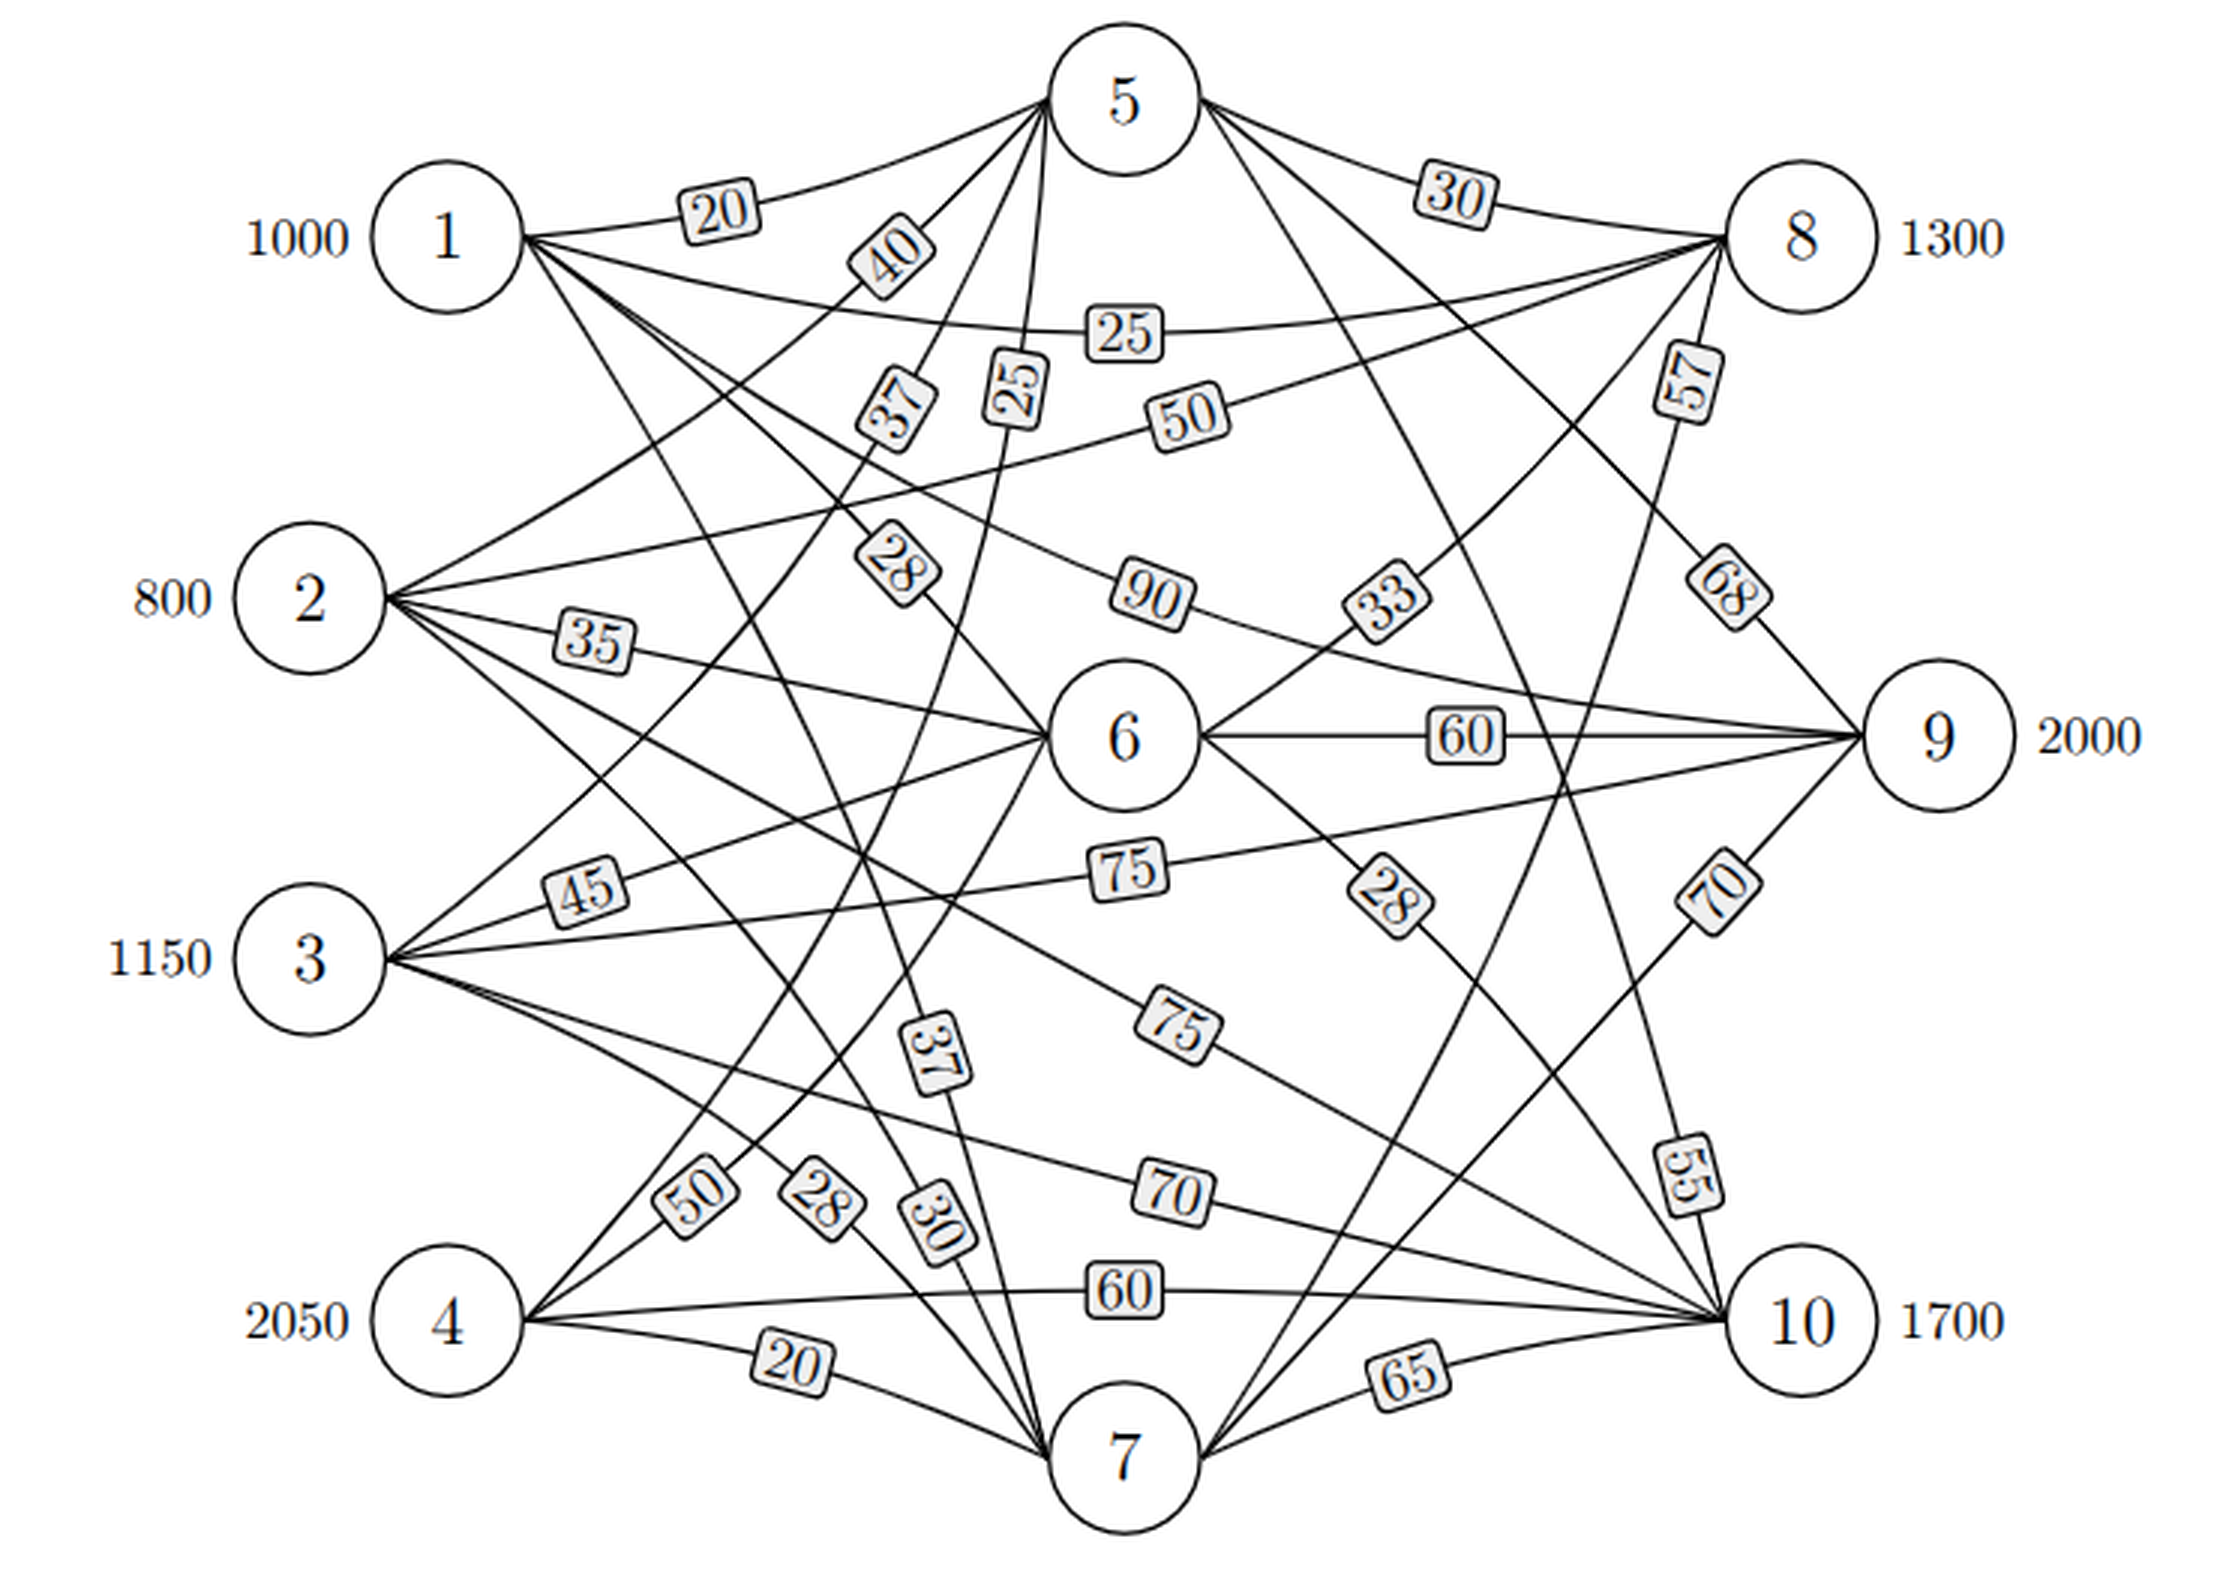
\includegraphics[width=0.92\textwidth]{figures/network-q1.png}
\captionof{figure}{Figure 1: The transport network (exact assignment diagram).}
\end{center}

Total supply \(=1000+800+1150+2050=5000\) and total demand \(=1300+2000+1700=5000\),
so the problem is \textbf{balanced}. Nodes 5, 6 and 7 are pure transshipment points:
goods may pass through them, but they have no net supply or demand of their own.

Reading every labelled arc in Figure~1 gives the following existing routes
(missing routes will later appear as \(M\) in the transportation tableau):
\begin{center}
\renewcommand{\arraystretch}{1.15}
\begin{tabular}{@{}lll@{}}
\toprule
From & To (unit costs) & \\
\midrule
1 & \(5\!:20\),\; \(6\!:28\),\; \(7\!:37\),\; \(9\!:90\) \\
2 & \(5\!:40\),\; \(6\!:35\),\; \(7\!:30\),\; \(8\!:25\),\; \(10\!:75\) \\
3 & \(5\!:37\),\; \(6\!:45\),\; \(7\!:28\),\; \(9\!:75\),\; \(10\!:70\) \\
4 & \(5\!:25\),\; \(6\!:50\),\; \(7\!:20\),\; \(10\!:60\) \\
5 & \(8\!:30\),\; \(9\!:68\),\; \(10\!:55\) \\
6 & \(8\!:33\),\; \(9\!:60\),\; \(10\!:28\) \\
7 & \(8\!:57\),\; \(9\!:70\),\; \(10\!:65\) \\
\bottomrule
\end{tabular}
\end{center}

% ----------------------------------------------------------------------
\PartHeading{(a) Mathematical model}
% ----------------------------------------------------------------------

\begin{ideabox}
We write one decision variable per existing arc, minimise total shipping cost, force
each source to ship out its supply, each destination to receive its demand, and each
intermediate node to \emph{balance} (inflow $=$ outflow).
\end{ideabox}

\Step{Decision variables}
For every arc \((i,j)\) that exists in the network, let
\[
  x_{ij} = \text{number of units shipped from node \(i\) to node \(j\)}.
\]
All \(x_{ij}\ge 0\). Forbidden (missing) arcs are simply omitted --- they never appear
as variables.

\Step{Objective function}
Minimise total transportation cost. Using the arc costs from the network:
\begin{align*}
\min\; Z =
&\; 20x_{15}+28x_{16}+37x_{17}+90x_{19} \\
&+40x_{25}+35x_{26}+30x_{27}+25x_{28}+75x_{2,10} \\
&+37x_{35}+45x_{36}+28x_{37}+75x_{39}+70x_{3,10} \\
&+25x_{45}+50x_{46}+20x_{47}+60x_{4,10} \\
&+30x_{58}+68x_{59}+55x_{5,10} \\
&+33x_{68}+60x_{69}+28x_{6,10} \\
&+57x_{78}+70x_{79}+65x_{7,10}.
\end{align*}
In compact form (summing only over existing arcs),
\[
  \min Z = \sum_{(i,j)\in\mathcal{A}} c_{ij}\, x_{ij}.
\]

\Step{Supply constraints (nodes 1--4)}
Everything that leaves a source must equal its available supply:
\begin{align*}
  x_{15}+x_{16}+x_{17}+x_{19} &= 1000, \\
  x_{25}+x_{26}+x_{27}+x_{28}+x_{2,10} &= 800, \\
  x_{35}+x_{36}+x_{37}+x_{39}+x_{3,10} &= 1150, \\
  x_{45}+x_{46}+x_{47}+x_{4,10} &= 2050.
\end{align*}

\Step{Intermediate / balance constraints (nodes 5--7)}
For a pure transshipment node, \textbf{inflow minus outflow equals zero}:
\begin{align*}
  (x_{15}+x_{25}+x_{35}+x_{45})-(x_{58}+x_{59}+x_{5,10}) &= 0, \\
  (x_{16}+x_{26}+x_{36}+x_{46})-(x_{68}+x_{69}+x_{6,10}) &= 0, \\
  (x_{17}+x_{27}+x_{37}+x_{47})-(x_{78}+x_{79}+x_{7,10}) &= 0.
\end{align*}

\Step{Demand constraints (nodes 8--10)}
\begin{align*}
  x_{28}+x_{58}+x_{68}+x_{78} &= 1300, \\
  x_{19}+x_{39}+x_{59}+x_{69}+x_{79} &= 2000, \\
  x_{2,10}+x_{3,10}+x_{4,10}+x_{5,10}+x_{6,10}+x_{7,10} &= 1700.
\end{align*}

\Step{Non-negativity}
\[
  x_{ij}\ge 0 \qquad\text{for every arc \((i,j)\)}.
\]

\begin{resultbox}[title={Part (a) --- model complete}]
The LP above is the complete transshipment formulation: objective, supply, balance,
demand, and non-negativity.
\end{resultbox}

% ----------------------------------------------------------------------
\PartHeading{(b) Standard transportation tableau}
% ----------------------------------------------------------------------

\begin{ideabox}
A transshipment problem becomes an ordinary transportation tableau by treating every
node that can ship as a \emph{row} and every node that can receive as a \emph{column},
and giving the intermediate nodes a large \textbf{buffer} \(B\) on both the supply and
demand sides. Shipments ``to yourself'' on the diagonal cost \(0\) and soak up unused buffer.
Missing arcs get cost \(M\) (forbidden).
\end{ideabox}

\Step{Choose the buffer}
\[
  B = \text{total external supply} = 5000.
\]
(Any \(B\) at least this large works; the course convention is to take exactly the total supply.)

\Step{Build the \(7\times 6\) cost matrix}
Rows \(=\) nodes \(1,2,3,4,5,6,7\) (all nodes that can ship).
Columns \(=\) nodes \(5,6,7,8,9,10\) (intermediates + destinations).
\begin{itemize}
  \item Diagonal cells \((5,5)\), \((6,6)\), \((7,7)\) have cost \(0\) (dummy / unused buffer).
  \item Existing arcs keep their unit costs.
  \item Non-existing arcs get cost \(M\).
\end{itemize}

\begin{center}
\renewcommand{\arraystretch}{1.35}
\begin{tabular}{|c|c|c|c|c|c|c|c|}
\hline
 & \textbf{5} & \textbf{6} & \textbf{7} & \textbf{8} & \textbf{9} & \textbf{10} & \textbf{Supply} \\
\hline
\textbf{1} & 20 & 28 & 37 & \(M\) & 90 & \(M\) & 1000 \\
\hline
\textbf{2} & 40 & 35 & 30 & 25 & \(M\) & 75 & 800 \\
\hline
\textbf{3} & 37 & 45 & 28 & \(M\) & 75 & 70 & 1150 \\
\hline
\textbf{4} & 25 & 50 & 20 & \(M\) & \(M\) & 60 & 2050 \\
\hline
\textbf{5} & 0 & \(M\) & \(M\) & 30 & 68 & 55 & 5000 \\
\hline
\textbf{6} & \(M\) & 0 & \(M\) & 33 & 60 & 28 & 5000 \\
\hline
\textbf{7} & \(M\) & \(M\) & 0 & 57 & 70 & 65 & 5000 \\
\hline
\textbf{Demand} & 5000 & 5000 & 5000 & 1300 & 2000 & 1700 & \(\mathbf{20000}\) \\
\hline
\end{tabular}
\end{center}

\begin{warningbox}
Check balance of the \emph{tableau}: total supply \(=1000+800+1150+2050+3\cdot 5000=20000\)
and total demand \(=3\cdot 5000+1300+2000+1700=20000\). A basic feasible solution of a
\(7\times 6\) tableau needs \(7+6-1=12\) basic cells.

This cost matrix is exactly the transcription of Figure~1: every labelled arc keeps its
unit cost, and every missing arc is \(M\). (It matches the class transportation tableau
built from the same figure.)
\end{warningbox}

\begin{resultbox}[title={Part (b)}]
The table above is the required standard transportation tableau.
\end{resultbox}

% ----------------------------------------------------------------------
\PartHeading{(c) IBFS by ADBAM}
% ----------------------------------------------------------------------

\begin{ideabox}
ADBAM always starts from the \emph{smallest remaining demand}, then fills the
\emph{cheapest open cell in that column}. After each allocation we update the leftover
supply/demand and either stay in the row, stay in the column, or restart --- exactly as
in Appendix~A.
\end{ideabox}

\Step{Start --- smallest demand}
The positive demands are \(5000,5000,5000,1300,2000,1700\). The unique minimum is
\textbf{column 8} with demand \(1300\).

In column~8 the finite costs are \(c_{28}=25\), \(c_{58}=30\), \(c_{68}=33\), \(c_{78}=57\).
Cheapest: cell \((2,8)\).

Allocate
\[
  x_{28}=\min(800,1300)=800.
\]
Row~2 is exhausted; column~8 still needs \(1300-800=500\).

\Step{Stay in column 8}
Next cheapest open row in column~8: cell \((5,8)\) with cost \(30\).
\[
  x_{58}=\min(5000,500)=500.
\]
Column~8 is done; row~5 still has \(4500\).

\Step{Stay in row 5}
Open columns for row~5: costs \(0,M,M,30,68,55\). Among columns with leftover demand,
the cheapest is \((5,5)\) with cost \(0\).
\[
  x_{55}=\min(4500,5000)=4500.
\]
Row~5 done; column~5 still needs \(500\).

\Step{Stay in column 5}
Next cheapest open row in column~5: \(c_{15}=20\) (then \(25,37,40,\ldots\)).
\[
  x_{15}=\min(1000,500)=500.
\]
Column~5 done; row~1 still has \(500\).

\Step{Stay in row 1}
Open columns for row~1 with leftover demand: \(c_{16}=28\), \(c_{17}=37\), \(c_{19}=90\).
Cheapest: \((1,6)\).
\[
  x_{16}=\min(500,5000)=500.
\]
Row~1 done; column~6 still needs \(4500\).

\Step{Stay in column 6}
Cheapest open cell: \((6,6)\) with cost \(0\).
\[
  x_{66}=\min(5000,4500)=4500.
\]
Column~6 done; row~6 still has \(500\).

\Step{Stay in row 6}
Open finite costs: \(c_{68}=33\), \(c_{69}=60\), \(c_{6,10}=28\). Cheapest: \((6,10)\).
\[
  x_{6,10}=\min(500,1700)=500.
\]
Row~6 done; column~10 still needs \(1200\).

\Step{Stay in column 10}
Open finite costs from rows with supply: \(c_{4,10}=60\), \(c_{3,10}=70\), \(c_{2,10}\) (row~2 empty),
\(c_{5,10}\) (row~5 empty), \(c_{7,10}=65\). Cheapest available: \((4,10)\).
\[
  x_{4,10}=\min(2050,1200)=1200.
\]
Column~10 done; row~4 still has \(850\).

\Step{Stay in row 4}
Open finite costs: \(c_{45}=25\) (col~5 done), \(c_{46}=50\) (col~6 done), \(c_{47}=20\).
Cheapest open: \((4,7)\).
\[
  x_{47}=\min(850,5000)=850.
\]
Row~4 done; column~7 still needs \(4150\).

\Step{Stay in column 7}
Cheapest open: \((7,7)\) with cost \(0\).
\[
  x_{77}=\min(5000,4150)=4150.
\]
Column~7 done; row~7 still has \(850\).

\Step{Stay in row 7 --- finish demand 9}
Open: \(c_{78}=57\) (col~8 done), \(c_{79}=70\), \(c_{7,10}\) (col~10 done).
\[
  x_{79}=\min(850,2000)=850.
\]
Row~7 done; column~9 still needs \(1150\).

\Step{Last allocation}
Only row~3 still has supply \(1150\), and column~9 needs \(1150\). Cell \((3,9)\) has cost \(75\):
\[
  x_{39}=1150.
\]
All supplies and demands are now zero.

\Step{Collect the IBFS and its cost}
The twelve basic allocations (exactly \(m+n-1\)) are:
\begin{center}
\begin{tabular}{@{}rrrr@{}}
\toprule
\(x_{ij}\) & Qty & \(c_{ij}\) & Contribution \\
\midrule
\(x_{15}\) & 500 & 20 & 10\,000 \\
\(x_{16}\) & 500 & 28 & 14\,000 \\
\(x_{28}\) & 800 & 25 & 20\,000 \\
\(x_{39}\) & 1150 & 75 & 86\,250 \\
\(x_{47}\) & 850 & 20 & 17\,000 \\
\(x_{4,10}\) & 1200 & 60 & 72\,000 \\
\(x_{55}\) & 4500 & 0 & 0 \\
\(x_{58}\) & 500 & 30 & 15\,000 \\
\(x_{66}\) & 4500 & 0 & 0 \\
\(x_{6,10}\) & 500 & 28 & 14\,000 \\
\(x_{77}\) & 4150 & 0 & 0 \\
\(x_{79}\) & 850 & 70 & 59\,500 \\
\midrule
 & & & \(\mathbf{Z_0=307\,750}\) \\
\bottomrule
\end{tabular}
\end{center}

\begin{notebox}
The diagonal buffer shipments \(x_{55},x_{66},x_{77}\) cost nothing --- they only balance the
tableau. The real physical flows are the other nine shipments.
\end{notebox}

\begin{resultbox}[title={Part (c) --- ADBAM IBFS}]
Initial basic feasible solution cost:
\[
  Z_0 = 307\,750.
\]
\end{resultbox}

% ----------------------------------------------------------------------
\PartHeading{(d) Optimal solution by the \(uv\) (MODI) method}
% ----------------------------------------------------------------------

\begin{ideabox}
For every \emph{basic} cell we solve \(u_i+v_j=c_{ij}\). Then for every \emph{empty} cell we
compute the opportunity cost \(k_{ij}=c_{ij}-u_i-v_j\). If all \(k_{ij}\ge 0\), the current
solution is optimal for a minimisation problem. If some \(k_{ij}<0\), that cell can improve
the cost and we enter it via a closed stepping-stone loop.
\end{ideabox}

\Step{Solve for duals on basic cells}
Set \(u_1=0\) (arbitrary but convenient). Working through the basic cells:
\begin{align*}
  u_1+v_5&=20 &&\Rightarrow && v_5=20,\\
  u_1+v_6&=28 &&\Rightarrow && v_6=28,\\
  u_5+v_5&=0 &&\Rightarrow && u_5=-20,\\
  u_5+v_8&=30 &&\Rightarrow && v_8=50,\\
  u_2+v_8&=25 &&\Rightarrow && u_2=-25,\\
  u_6+v_6&=0 &&\Rightarrow && u_6=-28,\\
  u_6+v_{10}&=28 &&\Rightarrow && v_{10}=56,\\
  u_4+v_{10}&=60 &&\Rightarrow && u_4=4,\\
  u_4+v_7&=20 &&\Rightarrow && v_7=16,\\
  u_7+v_7&=0 &&\Rightarrow && u_7=-16,\\
  u_7+v_9&=70 &&\Rightarrow && v_9=86,\\
  u_3+v_9&=75 &&\Rightarrow && u_3=-11.
\end{align*}

\begin{center}
\begin{tabular}{@{}ccccccc@{}}
\toprule
\(u_1\) & \(u_2\) & \(u_3\) & \(u_4\) & \(u_5\) & \(u_6\) & \(u_7\) \\
\midrule
0 & \(-25\) & \(-11\) & 4 & \(-20\) & \(-28\) & \(-16\) \\
\bottomrule
\end{tabular}
\qquad
\begin{tabular}{@{}cccccc@{}}
\toprule
\(v_5\) & \(v_6\) & \(v_7\) & \(v_8\) & \(v_9\) & \(v_{10}\) \\
\midrule
20 & 28 & 16 & 50 & 86 & 56 \\
\bottomrule
\end{tabular}
\end{center}

\Step{Evaluate every non-basic (finite-cost) cell}
\[
  k_{ij}=c_{ij}-u_i-v_j.
\]
\begin{center}
\begin{tabular}{@{}lrl@{}}
\toprule
Cell & Calculation & \(k_{ij}\) \\
\midrule
\((1,7)\) & \(37-0-16\) & \(+21\) \\
\((1,9)\) & \(90-0-86\) & \(+4\) \\
\((2,5)\) & \(40-(-25)-20\) & \(+45\) \\
\((2,6)\) & \(35-(-25)-28\) & \(+32\) \\
\((2,7)\) & \(30-(-25)-16\) & \(+39\) \\
\((2,10)\) & \(75-(-25)-56\) & \(+44\) \\
\((3,5)\) & \(37-(-11)-20\) & \(+28\) \\
\((3,6)\) & \(45-(-11)-28\) & \(+28\) \\
\((3,7)\) & \(28-(-11)-16\) & \(+23\) \\
\((3,10)\) & \(70-(-11)-56\) & \(+25\) \\
\((4,5)\) & \(25-4-20\) & \(+1\) \\
\((4,6)\) & \(50-4-28\) & \(+18\) \\
\((5,9)\) & \(68-(-20)-86\) & \(+2\) \\
\((5,10)\) & \(55-(-20)-56\) & \(+19\) \\
\((6,8)\) & \(33-(-28)-50\) & \(+11\) \\
\((6,9)\) & \(60-(-28)-86\) & \(+2\) \\
\((7,8)\) & \(57-(-16)-50\) & \(+23\) \\
\((7,10)\) & \(65-(-16)-56\) & \(+25\) \\
\bottomrule
\end{tabular}
\end{center}

\begin{warningbox}
All opportunity costs are \textbf{strictly positive}. For a cost-minimisation transportation
problem that means no empty cell can reduce \(Z\). The ADBAM solution is already optimal
--- no stepping-stone improvement is needed.
\end{warningbox}

\Step{Report the optimal shipments (physical arcs only)}
Dropping the zero-cost buffer loops, the optimal flow is:
\begin{align*}
  x_{15}&=500,&
  x_{16}&=500,&
  x_{28}&=800,&
  x_{39}&=1150,\\
  x_{47}&=850,&
  x_{4,10}&=1200,&
  x_{58}&=500,&
  x_{6,10}&=500,&
  x_{79}&=850.
\end{align*}
Quick sanity checks:
\begin{itemize}
  \item Node~5: in \(500\), out \(500\).
  \item Node~6: in \(500\), out \(500\).
  \item Node~7: in \(850\), out \(850\).
  \item Destinations: \(800+500=1300\), \(1150+850=2000\), \(1200+500=1700\).
\end{itemize}

\begin{resultbox}[title={Part (d) --- optimal solution}]
The \(uv\) test shows every \(k_{ij}\ge 0\), so the ADBAM IBFS is optimal with
\[
  Z^*=307\,750.
\]
\end{resultbox}
